\subsection{Vzdálenost bodu od přímky}
\label{subsec:Distance_point_line}

V předchozích částech jsme se zabývali různými způsoby vyjádření
přímky a vzájemnou polohou dvou přímek. Nyní se zaměříme na další
základní úlohu analytické geometrie: určení vzdálenosti bodu od
přímky.

Vzdálenost bodu od přímky využijeme například při výpočtu výšek
v trojúhelníku, při hledání bodů v předepsané vzdálenosti od dané
přímky nebo při určování vzdálenosti dvou rovnoběžných přímek.


\subsubsection{Geometrický význam vzdálenosti bodu od přímky}
\label{subsubsec:Geometric_meaning_distance_point_line}

Uvažujme bod $P$, který neleží na přímce $p$. Z bodu $P$ můžeme vést
k bodům přímky $p$ nekonečně mnoho úseček. Jejich délky však nejsou
stejné. Nejkratší z nich je úsečka, která je k přímce $p$ kolmá.

\begin{definition}\label{def:Distance_point_line}
    \textbf{Vzdáleností bodu $P$ od přímky $p$} nazýváme délku
    úsečky $PQ$, kde $Q$ je pata kolmice vedené z bodu $P$ na
    přímku $p$.

    Vzdálenost zapisujeme
    \[
        d(P,p)=|PQ|.
    \]
\end{definition}

Bod $Q$ nazýváme \textbf{kolmým průmětem bodu $P$ na přímku $p$}
nebo také \textbf{patou kolmice} z bodu $P$ na přímku $p$.

Jestliže bod $P$ na přímce $p$ leží, je jeho kolmým průmětem samotný
bod $P$ a platí
\[
    d(P,p)=0.
\]
Vzdálenost bodu od přímky je proto vždy nezáporné reálné číslo.

\begin{figure}[H]
    \centering
    \begin{tikzpicture}[scale=1.05]

        \coordinate (Q) at (0,0);
        \coordinate (P) at (-0.9,1.8);

        % Přímka p se směrovým vektorem (2;1)
        \draw[thin, <->] (-3,-1.5) -- (3,1.5)
            node[above right] {$p$};

        % Kolmice a vzdálenost
        \draw[dashed] (P) -- (Q);
        \node[left] at (-0.48,0.92) {$d(P,p)$};

        % Body
        \fill (P) circle (2.5pt) node[above left] {$P$};
        \fill (Q) circle (2.5pt) node[below right] {$Q$};

        % Pravý úhel
        \draw
            (-0.18,0.09)
            --
            (-0.27,0.27)
            --
            (-0.09,0.36);

    \end{tikzpicture}
    \caption{Vzdálenost bodu $P$ od přímky $p$ je délka kolmice
    vedené z bodu $P$ na přímku $p$.}
    \label{fig:Geometric_distance_point_line}
\end{figure}


\subsubsection{Odvození vzorce pro vzdálenost bodu od přímky}
\label{subsubsec:Derivation_distance_point_line}

Uvažujme bod
\[
    P[x_P;y_P]
\]
a přímku zadanou obecnou rovnicí
\begin{equation}\label{eq:Distance_general_line}
    p:\quad ax+by+c=0,
    \qquad
    (a;b)\neq(0;0).
\end{equation}

Normálový vektor přímky $p$ je
\[
    \vec{n}_p=(a;b).
\]
Přímka kolmá k přímce $p$ proto může mít tento normálový vektor jako
svůj směrový vektor. Označme tuto kolmici písmenem $q$. Protože má
procházet bodem $P[x_P;y_P]$, její parametrické vyjádření je
\begin{equation}\label{eq:Perpendicular_through_point_distance}
    \begin{aligned}
        q:\quad x&=x_P+at,\\
                 y&=y_P+bt,
                 \qquad t\in\mathbb{R}.
    \end{aligned}
\end{equation}

Průsečík přímek $p$ a $q$ je pata kolmice $Q$. Jeho parametr určíme
dosazením parametrického vyjádření přímky $q$ do obecné rovnice
přímky $p$:
\begin{align*}
    a(x_P+at)+b(y_P+bt)+c&=0,\\
    ax_P+a^2t+by_P+b^2t+c&=0,\\
    (a^2+b^2)t+ax_P+by_P+c&=0.
\end{align*}

Protože $(a;b)\neq(0;0)$, platí
\[
    a^2+b^2>0,
\]
a můžeme vyjádřit parametr
\begin{equation}\label{eq:Parameter_foot_point_line}
    t_0
    =
    -\frac{ax_P+by_P+c}{a^2+b^2}.
\end{equation}

Pata kolmice má tedy souřadnice
\begin{equation}\label{eq:Foot_point_general_line}
    Q\left[
        x_P-a\frac{ax_P+by_P+c}{a^2+b^2};
        y_P-b\frac{ax_P+by_P+c}{a^2+b^2}
    \right].
\end{equation}

Vektor směřující z bodu $P$ do bodu $Q$ je násobkem normálového
vektoru:
\[
    \overrightarrow{PQ}
    =
    t_0(a;b).
\]
Jeho velikost je
\begin{align*}
    |PQ|
    &=
    |t_0|\sqrt{a^2+b^2}\\
    &=
    \left|
        -\frac{ax_P+by_P+c}{a^2+b^2}
    \right|
    \sqrt{a^2+b^2}\\
    &=
    \frac{|ax_P+by_P+c|}{\sqrt{a^2+b^2}}.
\end{align*}

Dostáváme tak základní vzorec pro vzdálenost bodu od přímky.

Pro bod $P[x_P;y_P]$ a přímku
\[
    p:\quad ax+by+c=0,
    \qquad
    (a;b)\neq(0;0),
\]
tedy platí
\begin{equation}\label{eq:Distance_point_general_line}
    d(P,p)
    =
    \frac{|ax_P+by_P+c|}{\sqrt{a^2+b^2}}.
\end{equation}

\begin{remark}\label{rem:Meaning_distance_formula_parts}
    Čitatel vzorce
    \[
        |ax_P+by_P+c|
    \]
    získáme dosazením souřadnic bodu $P$ do levé strany obecné
    rovnice přímky. Leží-li bod na přímce, vyjde tento výraz roven
    nule.

    Hodnota výrazu však závisí na délce použitého normálového vektoru.
    Proto ji dělíme velikostí normálového vektoru
    \[
        |\vec{n}_p|=\sqrt{a^2+b^2}.
    \]
    Tím výsledek nezávisí na tom, kterým ekvivalentním zápisem obecné
    rovnice je přímka vyjádřena.
\end{remark}

Skutečně, vynásobíme-li obecnou rovnici nenulovým číslem
$\lambda$, dostaneme
\[
    \lambda ax+\lambda by+\lambda c=0.
\]
Po dosazení do vzorce pro vzdálenost získáme
\begin{align*}
    \frac{|\lambda ax_P+\lambda by_P+\lambda c|}
    {\sqrt{(\lambda a)^2+(\lambda b)^2}}
    &=
    \frac{|\lambda|\,|ax_P+by_P+c|}
    {|\lambda|\sqrt{a^2+b^2}}\\
    &=
    \frac{|ax_P+by_P+c|}{\sqrt{a^2+b^2}}.
\end{align*}
Vzdálenost se tedy nezmění.

\begin{example}\label{exa:Basic_distance_point_line}
    Určete vzdálenost bodu
    \[
        P[-4;2]
    \]
    od přímky
    \[
        p:\quad 3x-4y-5=0.
    \]

    Dosadíme do vztahu \eqref{eq:Distance_point_general_line}:
    \begin{align*}
        d(P,p)
        &=
        \frac{|3\cdot(-4)-4\cdot2-5|}
        {\sqrt{3^2+(-4)^2}}\\
        &=
        \frac{|-12-8-5|}{\sqrt{9+16}}\\
        &=
        \frac{25}{5}\\
        &=5.
    \end{align*}

    Vzdálenost bodu $P$ od přímky $p$ je tedy
    \[
        d(P,p)=5.
    \]

    Určíme také patu kolmice. Normálový vektor přímky
    \[
        \vec{n}_p=(3;-4)
    \]
    použijeme jako směrový vektor kolmice procházející bodem $P$:
    \[
        \begin{aligned}
            q:\quad x&=-4+3t,\\
                     y&=2-4t,
                     \qquad t\in\mathbb{R}.
        \end{aligned}
    \]

    Po dosazení do rovnice přímky $p$ dostáváme
    \begin{align*}
        3(-4+3t)-4(2-4t)-5&=0,\\
        -12+9t-8+16t-5&=0,\\
        25t-25&=0,\\
        t&=1.
    \end{align*}

    Pata kolmice je proto bod
    \[
        Q[-1;-2].
    \]
    Ověření pomocí vzdálenosti bodů dává
    \[
        |PQ|
        =
        \sqrt{(-1-(-4))^2+(-2-2)^2}
        =
        \sqrt{3^2+(-4)^2}
        =5.
    \]
\end{example}


\subsubsection{Vzdálenost v jednotlivých tvarech rovnice přímky}
\label{subsubsec:Distance_point_line_forms}

Základní vztah \eqref{eq:Distance_point_general_line} používá obecnou
rovnici přímky. Je-li přímka zadána jiným způsobem, můžeme ji převést
do obecného tvaru. Z převodů však lze také odvodit vzorce použitelné
přímo pro parametrické a směrnicové vyjádření.

\paragraph{Přímka zadaná obecnou rovnicí}

Pro přímku
\[
    p:\quad ax+by+c=0
\]
a bod $P[x_P;y_P]$ přímo používáme vztah
\[
    d(P,p)
    =
    \frac{|ax_P+by_P+c|}{\sqrt{a^2+b^2}}.
\]

\paragraph{Přímka ve směrnicovém tvaru}

Směrnicový tvar
\[
    p:\quad y=kx+q
\]
převedeme do obecné rovnice
\[
    kx-y+q=0.
\]
Proto platí
\begin{equation}\label{eq:Distance_point_slope_line}
    d(P,p)
    =
    \frac{|kx_P-y_P+q|}{\sqrt{k^2+1}}.
\end{equation}

\begin{example}\label{exa:Distance_point_slope_line}
    Určete vzdálenost bodu
    \[
        A[2;-1]
    \]
    od přímky
    \[
        p:\quad y=\frac12x+3.
    \]

    Použijeme vztah \eqref{eq:Distance_point_slope_line}:
    \begin{align*}
        d(A,p)
        &=
        \frac{
            \left|
                \frac12\cdot2-(-1)+3
            \right|
        }
        {\sqrt{\left(\frac12\right)^2+1}}\\
        &=
        \frac{|1+1+3|}{\sqrt{\frac14+1}}\\
        &=
        \frac{5}{\frac{\sqrt5}{2}}\\
        &=
        2\sqrt5.
    \end{align*}

    Ke stejnému výsledku dospějeme po převodu přímky do obecného
    tvaru
    \[
        x-2y+6=0.
    \]
\end{example}

\paragraph{Přímka zadaná parametricky}

Uvažujme přímku
\[
    \begin{aligned}
        p:\quad x&=x_A+t u_x,\\
                 y&=y_A+t u_y,
                 \qquad t\in\mathbb{R},
    \end{aligned}
\]
která prochází bodem $A[x_A;y_A]$ a má směrový vektor
\[
    \vec{u}=(u_x;u_y).
\]

Její obecná rovnice může mít tvar
\[
    u_y(x-x_A)-u_x(y-y_A)=0.
\]
Dosazením do vztahu pro vzdálenost dostáváme
\begin{equation}\label{eq:Distance_point_parametric_line}
    d(P,p)
    =
    \frac{
        |u_y(x_P-x_A)-u_x(y_P-y_A)|
    }
    {\sqrt{u_x^2+u_y^2}}.
\end{equation}

\begin{remark}\label{rem:Area_interpretation_parametric_distance}
    Čitatel vztahu \eqref{eq:Distance_point_parametric_line} odpovídá
    obsahu rovnoběžníku určeného směrovým vektorem $\vec{u}$ a
    vektorem $\overrightarrow{AP}$. Vydělíme-li tento obsah délkou
    základny $|\vec{u}|$, získáme výšku rovnoběžníku, tedy vzdálenost
    bodu $P$ od přímky $p$.
\end{remark}

\begin{example}\label{exa:Distance_point_parametric_line}
    Určete vzdálenost bodu
    \[
        P[4;1]
    \]
    od přímky
    \[
        \begin{aligned}
            p:\quad x&=1+2t,\\
                     y&=-1+t,
                     \qquad t\in\mathbb{R}.
        \end{aligned}
    \]

    Přímka prochází bodem $A[1;-1]$ a má směrový vektor
    \[
        \vec{u}=(2;1).
    \]
    Použijeme vztah \eqref{eq:Distance_point_parametric_line}:
    \begin{align*}
        d(P,p)
        &=
        \frac{|1(4-1)-2(1-(-1))|}{\sqrt{2^2+1^2}}\\
        &=
        \frac{|3-4|}{\sqrt5}\\
        &=
        \frac{1}{\sqrt5}.
    \end{align*}
\end{example}

\begin{remark}\label{rem:General_method_distance_point_line}
    Vztahy pro vzdálenost bodu od přímky zadané směrnicově nebo
    parametricky není nutné pamatovat jako samostatné vzorce.
    Přímku můžeme vždy nejprve převést na obecnou rovnici a následně
    použít vztah \eqref{eq:Distance_point_general_line}.

    Tento postup je univerzální a lze jej použít pro každou přímku
    v rovině. Vztahy odvozené přímo pro směrnicový nebo parametrický
    tvar představují pouze zkrácený postup.
\end{remark}


\subsubsection{Body v předepsané vzdálenosti od přímky}
\label{subsubsec:Points_given_distance_line}

Vzorec pro vzdálenost můžeme použít také obráceně. Neznáme-li bod,
ale známe podmínku, kterou musí splňovat, dosadíme jeho neznámé
souřadnice do vztahu pro vzdálenost. Vznikne rovnice, zpravidla
s absolutní hodnotou.

Absolutní hodnotu nesmíme při řešení vynechat. Body mohou ležet na
obou stranách přímky, a proto úloha často vede ke dvěma řešením.

\begin{example}\label{exa:Point_on_x_axis_given_distance}
    Na ose $x$ najděte všechny body, jejichž vzdálenost od přímky
    \[
        p:\quad x-2y+2=0
    \]
    je rovna $\sqrt5$.

    Hledaný bod leží na ose $x$, a proto má tvar
    \[
        A[a;0].
    \]

    Dosadíme jeho souřadnice do vzorce pro vzdálenost:
    \begin{align*}
        \frac{|a-2\cdot0+2|}{\sqrt{1^2+(-2)^2}}
        &=
        \sqrt5,\\
        \frac{|a+2|}{\sqrt5}
        &=
        \sqrt5,\\
        |a+2|&=5.
    \end{align*}

    Rovnice s absolutní hodnotou má dvě řešení:
    \[
        a+2=5
        \qquad\text{nebo}\qquad
        a+2=-5.
    \]
    Odtud
    \[
        a_1=3,
        \qquad
        a_2=-7.
    \]

    Hledanými body jsou
    \[
        A_1[3;0]
        \qquad\text{a}\qquad
        A_2[-7;0].
    \]

    Situace je znázorněna na obrázku
    \ref{fig:Points_on_x_axis_given_distance}. Přerušované přímky
    tvoří množinu všech bodů, které mají od přímky $p$ vzdálenost
    $\sqrt5$.

    \begin{figure}[H]
        \centering
        \begin{tikzpicture}[scale=0.65]

            % Osy
            \draw[<->] (-9,0) -- (6,0) node[right] {$x$};
            \draw[<->] (0,-3) -- (0,5) node[above] {$y$};
            \node[below right] at (0,0) {$O$};

            % Přímka p: y=0.5x+1
            \draw[thick, <->] (-8,-3) -- (6,4)
                node[above right] {$p$};

            % Rovnoběžky ve vzdálenosti sqrt(5)
            % x-2y-3=0 -> y=0.5x-1.5
            \draw[dashed, <->] (-3, -3) -- (6,1.5);
            % x-2y+7=0 -> y=0.5x+3.5
            \draw[dashed, <->] (-9,-1) -- (3,5);

            % Body na ose x
            \fill (3,0) circle (3pt) node[below right] {$A_1[3;0]$};
            \fill (-7,0) circle (3pt) node[below left] {$A_2[-7;0]$};

        \end{tikzpicture}
        \caption{Na ose $x$ leží dva body ve vzdálenosti $\sqrt5$
        od přímky $p:x-2y+2=0$.}
        \label{fig:Points_on_x_axis_given_distance}
    \end{figure}
\end{example}

\begin{example}\label{exa:Point_on_line_given_distance_from_line}
    Na přímce
    \[
        q:\quad x+3y-1=0
    \]
    najděte všechny body, které mají od přímky
    \[
        p:\quad 2x+y-7=0
    \]
    vzdálenost $2\sqrt5$.

    Označme hledaný bod
    \[
        A[x;y].
    \]
    Musí splňovat dvě podmínky:
    \begin{enumerate}
        \item bod $A$ leží na přímce $q$,
        \item vzdálenost bodu $A$ od přímky $p$ je $2\sqrt5$.
    \end{enumerate}

    Z první podmínky dostáváme
    \[
        x+3y-1=0,
    \]
    tedy
    \[
        x=1-3y.
    \]

    Druhou podmínku zapíšeme pomocí vzorce pro vzdálenost:
    \begin{align*}
        \frac{|2x+y-7|}{\sqrt{2^2+1^2}}
        &=
        2\sqrt5,\\
        |2x+y-7|&=10.
    \end{align*}

    Dosadíme $x=1-3y$:
    \begin{align*}
        |2(1-3y)+y-7|&=10,\\
        |-5y-5|&=10,\\
        |y+1|&=2.
    \end{align*}

    Dostáváme dvě možnosti:
    \[
        y_1=1
        \qquad\text{nebo}\qquad
        y_2=-3.
    \]

    Odpovídající první souřadnice jsou
    \[
        x_1=1-3\cdot1=-2,
    \]
    \[
        x_2=1-3\cdot(-3)=10.
    \]

    Hledané body jsou
    \[
        A_1[-2;1]
        \qquad\text{a}\qquad
        A_2[10;-3].
    \]
\end{example}


\subsubsection{Vzdálenost rovnoběžných přímek}
\label{subsubsec:Distance_parallel_lines}

Vzdálenost dvou různých rovnoběžných přímek definujeme jako
vzdálenost libovolného bodu jedné přímky od přímky druhé. Tato
vzdálenost je podél obou přímek stále stejná. U různoběžných přímek
se vzdálenost v tomto smyslu neurčuje; jejich nejmenší možná
vzdálenost je nulová, protože mají společný bod.

Uvažujme rovnoběžné přímky zapsané se stejnými koeficienty u
proměnných $x$ a $y$:
\[
    p:\quad ax+by+c_1=0,
\]
\[
    q:\quad ax+by+c_2=0.
\]

Zvolme libovolný bod $Q[x_Q;y_Q]$ přímky $q$. Protože na této přímce
leží, platí
\[
    ax_Q+by_Q+c_2=0,
\]
a tedy
\[
    ax_Q+by_Q=-c_2.
\]

Vzdálenost bodu $Q$ od přímky $p$ je
\begin{align*}
    d(Q,p)
    &=
    \frac{|ax_Q+by_Q+c_1|}{\sqrt{a^2+b^2}}\\
    &=
    \frac{|-c_2+c_1|}{\sqrt{a^2+b^2}}\\
    &=
    \frac{|c_1-c_2|}{\sqrt{a^2+b^2}}.
\end{align*}

Tato hodnota nezávisí na volbě bodu $Q$, a je proto vzdáleností obou
přímek.

Jsou-li dvě různé rovnoběžné přímky zapsány ve tvaru
\[
    p:\quad ax+by+c_1=0
\]
a
\[
    q:\quad ax+by+c_2=0,
\]
potom je jejich vzdálenost
\begin{equation}\label{eq:Distance_parallel_lines}
    d(p,q)
    =
    \frac{|c_1-c_2|}{\sqrt{a^2+b^2}}.
\end{equation}

\begin{remark}\label{rem:Same_normal_parallel_distance}
    Vztah \eqref{eq:Distance_parallel_lines} můžeme použít přímo pouze
    tehdy, když mají obě rovnice stejné koeficienty $a$ a $b$.
    Jsou-li jejich normálové vektory pouze rovnoběžné, musíme nejprve
    jednu z rovnic vynásobit vhodným nenulovým číslem.
\end{remark}

\begin{example}\label{exa:Parallel_lines_given_distance}
    Najděte všechny přímky, které jsou rovnoběžné s přímkou
    \[
        p:\quad x-3y+2=0
    \]
    a mají od ní vzdálenost $\sqrt{10}$.

    Každá přímka rovnoběžná s přímkou $p$ může být zapsána ve tvaru
    \[
        q:\quad x-3y+c=0.
    \]

    Použijeme vztah pro vzdálenost rovnoběžných přímek:
    \begin{align*}
        \frac{|c-2|}{\sqrt{1^2+(-3)^2}}
        &=
        \sqrt{10},\\
        \frac{|c-2|}{\sqrt{10}}
        &=
        \sqrt{10},\\
        |c-2|&=10.
    \end{align*}

    Odtud
    \[
        c_1=12,
        \qquad
        c_2=-8.
    \]

    Hledané přímky jsou
    \[
        q_1:\quad x-3y+12=0
    \]
    a
    \[
        q_2:\quad x-3y-8=0.
    \]

    Existují tedy právě dvě takové přímky, jedna na každé straně
    původní přímky $p$.
\end{example}

\begin{example}\label{exa:Midline_parallel_strip}
    Jsou dány rovnoběžné přímky
    \[
        p:\quad x-2y+6=0
    \]
    a
    \[
        q:\quad 2x-4y-5=0.
    \]
    Určete rovnoběžnou přímku, která má od obou přímek stejnou
    vzdálenost.

    Nejprve upravíme rovnici přímky $p$ tak, aby obě rovnice měly
    stejné koeficienty u $x$ a $y$:
    \[
        p:\quad 2x-4y+12=0.
    \]

    Hledaná přímka má tvar
    \[
        r:\quad 2x-4y+c=0.
    \]
    Podmínka stejné vzdálenosti je
    \[
        \frac{|c-12|}{\sqrt{2^2+(-4)^2}}
        =
        \frac{|c-(-5)|}{\sqrt{2^2+(-4)^2}}.
    \]
    Po zkrácení společného jmenovatele dostáváme
    \[
        |c-12|=|c+5|.
    \]

    Číslo $c$ musí ležet přesně uprostřed mezi čísly $12$ a $-5$:
    \[
        c
        =
        \frac{12+(-5)}{2}
        =
        \frac72.
    \]

    Hledaná přímka je
    \[
        r:\quad 2x-4y+\frac72=0.
    \]
    Po vynásobení rovnice číslem $2$ ji můžeme zapsat také jako
    \[
        r:\quad 4x-8y+7=0.
    \]
\end{example}


\subsubsection{Body stejně vzdálené od dvou přímek}
\label{subsubsec:Points_equidistant_two_lines}

Uvažujme dvě přímky
\[
    p:\quad a_1x+b_1y+c_1=0
\]
a
\[
    q:\quad a_2x+b_2y+c_2=0.
\]
Hledáme všechny body $X[x;y]$, které mají od obou přímek stejnou
vzdálenost. Musí tedy platit
\begin{equation}\label{eq:Equidistant_two_lines_absolute}
    \frac{|a_1x+b_1y+c_1|}{\sqrt{a_1^2+b_1^2}}
    =
    \frac{|a_2x+b_2y+c_2|}{\sqrt{a_2^2+b_2^2}}.
\end{equation}

Rovnost absolutních hodnot vede ke dvěma možnostem:
\begin{equation}\label{eq:Angle_bisectors_general}
    \frac{a_1x+b_1y+c_1}{\sqrt{a_1^2+b_1^2}}
    =
    \pm
    \frac{a_2x+b_2y+c_2}{\sqrt{a_2^2+b_2^2}}.
\end{equation}

Jsou-li přímky různoběžné, popisují obě vzniklé rovnice osy úhlů,
které přímky svírají. Každý bod osy úhlu má totiž od obou ramen úhlu
stejnou vzdálenost. Situace je znázorněna na obrázku
\ref{fig:Angle_bisectors_equidistant_lines}.

\begin{figure}[H]
    \centering
    \begin{tikzpicture}[scale=0.85]

        \coordinate (O) at (0,0);

        % Původní přímky
        \draw[thin, <->] (-3.3,0) -- (3.3,0)
            node[right] {$p$};
        \draw[thin, <->] (-1.8,-3.12) -- (1.8,3.12)
            node[above right] {$q$};

        % Osy úhlů
        \draw[dashed, <->] (-3,-1.73) -- (3,1.73)
            node[above right] {$o_1$};
        \draw[dashed, <->] (-1.5,2.60) -- (1.5,-2.60)
            node[below right] {$o_2$};

        \fill (O) circle (2.5pt) node[below left] {$O$};

    \end{tikzpicture}
    \caption{Body stejně vzdálené od dvou různoběžných přímek leží
    na osách úhlů $o_1$ a $o_2$.}
    \label{fig:Angle_bisectors_equidistant_lines}
\end{figure}

\begin{example}\label{exa:Angle_bisectors_from_distance}
    Najděte všechny body roviny, které mají stejnou vzdálenost od
    přímek
    \[
        p:\quad x+2y-3=0
    \]
    a
    \[
        q:\quad 2x-y-1=0.
    \]

    Velikosti normálových vektorů obou přímek jsou stejné:
    \[
        \sqrt{1^2+2^2}
        =
        \sqrt{2^2+(-1)^2}
        =
        \sqrt5.
    \]
    Podmínka stejné vzdálenosti se proto zjednoduší na
    \[
        |x+2y-3|
        =
        |2x-y-1|.
    \]

    Dostáváme dvě lineární rovnice.

    První možnost:
    \begin{align*}
        x+2y-3&=2x-y-1,\\
        -x+3y-2&=0,\\
        x-3y+2&=0.
    \end{align*}

    Druhá možnost:
    \begin{align*}
        x+2y-3&=-(2x-y-1),\\
        x+2y-3&=-2x+y+1,\\
        3x+y-4&=0.
    \end{align*}

    Množinu všech bodů stejně vzdálených od přímek $p$ a $q$ tedy
    tvoří dvě přímky
    \[
        o_1:\quad x-3y+2=0
    \]
    a
    \[
        o_2:\quad 3x+y-4=0.
    \]
    Jsou to osy obou úhlů, které přímky $p$ a $q$ svírají.
\end{example}

\begin{remark}\label{rem:Equidistant_parallel_lines}
    Jsou-li původní přímky rovnoběžné a různé, množinu bodů stejně
    vzdálených od obou přímek tvoří jediná přímka ležící uprostřed
    pásu mezi nimi. Tuto situaci jsme řešili v příkladu
    \ref{exa:Midline_parallel_strip}.
\end{remark}


\subsubsection{Souhrnný příklad s trojúhelníkem}
\label{subsubsec:Distance_triangle_summary}

\begin{example}\label{exa:Distance_triangle_altitudes_area}
    Je dán trojúhelník $ABC$ s vrcholy
    \[
        A[2;-1],
        \qquad
        B[1;4],
        \qquad
        C[-3;-3].
    \]
    Určete:
    \begin{enumerate}[label=\alph*)]
        \item výšku $v_c$ na stranu $AB$,
        \item výšku $v_b$ na stranu $AC$,
        \item obsah trojúhelníku dvěma způsoby.
    \end{enumerate}

    \begin{enumerate}[label=\alph*), leftmargin=2em]
        \item \textbf{Výška $v_c$}

        Výška $v_c$ je vzdálenost vrcholu $C$ od přímky obsahující
        stranu $AB$.

        Směrový vektor strany $AB$ je
        \[
            \overrightarrow{AB}
            =
            (1-2;4-(-1))
            =
            (-1;5).
        \]
        Jako normálový vektor přímky $AB$ zvolíme
        \[
            \vec{n}_{AB}=(5;1).
        \]
        Obecná rovnice má tvar
        \[
            5x+y+c=0.
        \]
        Dosazením bodu $A[2;-1]$ získáme
        \begin{align*}
            5\cdot2+(-1)+c&=0,\\
            c&=-9.
        \end{align*}
        Přímka $AB$ má tedy rovnici
        \[
            5x+y-9=0.
        \]

        Výška je
        \begin{align*}
            v_c
            &=
            d(C,AB)\\
            &=
            \frac{|5\cdot(-3)+(-3)-9|}{\sqrt{5^2+1^2}}\\
            &=
            \frac{27}{\sqrt{26}}.
        \end{align*}

        \item \textbf{Výška $v_b$}

        Výška $v_b$ je vzdálenost vrcholu $B$ od přímky obsahující
        stranu $AC$.

        Směrový vektor strany $AC$ je
        \[
            \overrightarrow{AC}
            =
            (-3-2;-3-(-1))
            =
            (-5;-2).
        \]
        Jako normálový vektor zvolíme
        \[
            \vec{n}_{AC}=(2;-5).
        \]
        Obecná rovnice má tvar
        \[
            2x-5y+c=0.
        \]
        Dosazením bodu $A[2;-1]$ dostáváme
        \begin{align*}
            2\cdot2-5\cdot(-1)+c&=0,\\
            c&=-9.
        \end{align*}
        Přímka $AC$ má rovnici
        \[
            2x-5y-9=0.
        \]

        Výška je
        \begin{align*}
            v_b
            &=
            d(B,AC)\\
            &=
            \frac{|2\cdot1-5\cdot4-9|}{\sqrt{2^2+(-5)^2}}\\
            &=
            \frac{27}{\sqrt{29}}.
        \end{align*}

        \item \textbf{Obsah trojúhelníku}

        Délka strany $AB$ je
        \[
            |AB|
            =
            \sqrt{(-1)^2+5^2}
            =
            \sqrt{26}.
        \]
        Proto
        \[
            S_{ABC}
            =
            \frac12|AB|v_c
            =
            \frac12\sqrt{26}\cdot\frac{27}{\sqrt{26}}
            =
            \frac{27}{2}.
        \]

        Délka strany $AC$ je
        \[
            |AC|
            =
            \sqrt{(-5)^2+(-2)^2}
            =
            \sqrt{29}.
        \]
        Druhým způsobem dostáváme
        \[
            S_{ABC}
            =
            \frac12|AC|v_b
            =
            \frac12\sqrt{29}\cdot\frac{27}{\sqrt{29}}
            =
            \frac{27}{2}.
        \]

        Oba výpočty vedou ke stejnému výsledku, což zároveň ověřuje
        správnost vypočítaných výšek.
    \end{enumerate}
\end{example}

Vzorec pro vzdálenost bodu od přímky tak propojuje obecnou rovnici
přímky, normálový vektor, kolmici i vzdálenost dvou bodů. Zároveň
umožňuje převést řadu geometrických úloh na řešení rovnic a soustav
rovnic.

\begin{example}\label{exa:Points_equidistant_from_triangle_side_lines}
    Je dán trojúhelník $ABC$ s vrcholy
    \[
        A[1;1],
        \qquad
        B[7;1],
        \qquad
        C[1;9].
    \]

    Určete všechny body $X[x;y]$ v rovině, které mají stejnou
    vzdálenost od všech tří přímek, na nichž leží strany
    trojúhelníku $ABC$.

    U každého nalezeného bodu určete tuto společnou vzdálenost
    a rozhodněte, který z bodů leží uvnitř trojúhelníku.

    Nejprve určíme obecné rovnice přímek, na nichž leží jednotlivé
    strany trojúhelníku.

    Přímka obsahující stranu $AB$ je vodorovná a prochází body
    $A[1;1]$ a $B[7;1]$. Její rovnice je
    \[
        p_{AB}:y-1=0.
    \]

    Přímka obsahující stranu $AC$ je svislá a prochází body
    $A[1;1]$ a $C[1;9]$. Její rovnice je
    \[
        p_{AC}:x-1=0.
    \]

    Pro přímku obsahující stranu $BC$ nejprve určíme směrový vektor
    \[
        \overrightarrow{BC}
        =
        (1-7;9-1)
        =
        (-6;8).
    \]
    Použijeme jednodušší směrový vektor
    \[
        \vec{u}_{BC}=(-3;4).
    \]
    K němu zvolíme normálový vektor
    \[
        \vec{n}_{BC}=(4;3).
    \]

    Přímka prochází bodem $B[7;1]$, a proto
    \begin{align*}
        4(x-7)+3(y-1)&=0,\\
        4x-28+3y-3&=0,\\
        4x+3y-31&=0.
    \end{align*}

    Dostáváme tedy tři přímky
    \[
        p_{AB}:y-1=0,
    \]
    \[
        p_{AC}:x-1=0,
    \]
    \[
        p_{BC}:4x+3y-31=0.
    \]

    Uvažujme nyní hledaný bod
    \[
        X[x;y].
    \]

    Podle vztahu \eqref{eq:Distance_point_general_line} je jeho
    vzdálenost od přímky $p_{AB}$ rovna
    \[
        d(X,p_{AB})
        =
        \frac{|y-1|}{\sqrt{0^2+1^2}}
        =
        |y-1|.
    \]

    Vzdálenost od přímky $p_{AC}$ je
    \[
        d(X,p_{AC})
        =
        \frac{|x-1|}{\sqrt{1^2+0^2}}
        =
        |x-1|.
    \]

    Vzdálenost od přímky $p_{BC}$ je
    \[
        d(X,p_{BC})
        =
        \frac{|4x+3y-31|}{\sqrt{4^2+3^2}}
        =
        \frac{|4x+3y-31|}{5}.
    \]

    Hledáme body, které mají od všech tří přímek stejnou vzdálenost.
    Musí proto platit
    \begin{equation}\label{eq:Equal_distances_triangle_side_lines}
        |x-1|
        =
        |y-1|
        =
        \frac{|4x+3y-31|}{5}.
    \end{equation}

    Nejprve vyřešíme podmínku
    \[
        |x-1|=|y-1|.
    \]

    Pro rovnost absolutních hodnot mohou nastat dvě možnosti:
    \[
        x-1=y-1
    \]
    nebo
    \[
        x-1=-(y-1).
    \]

    Získáváme tedy dvě přímky
    \[
        y=x
    \]
    a
    \[
        y=2-x.
    \]

    Tyto dvě přímky jsou osami úhlů přímek $p_{AB}$ a $p_{AC}$.
    Hledané body však musí mít stejnou vzdálenost také od přímky
    $p_{BC}$.

    \paragraph{První případ: $y=x$}

    Dosadíme $y=x$ do vztahu
    \eqref{eq:Equal_distances_triangle_side_lines}:
    \begin{align*}
        |x-1|
        &=
        \frac{|4x+3x-31|}{5},\\
        |x-1|
        &=
        \frac{|7x-31|}{5},\\
        5|x-1|
        &=
        |7x-31|.
    \end{align*}

    Rovnost absolutních hodnot můžeme zapsat jako
    \[
        7x-31=5(x-1)
    \]
    nebo
    \[
        7x-31=-5(x-1).
    \]

    Z první rovnice získáme
    \begin{align*}
        7x-31&=5x-5,\\
        2x&=26,\\
        x&=13.
    \end{align*}

    Protože $y=x$, dostáváme bod
    \[
        X_1[13;13].
    \]

    Z druhé rovnice získáme
    \begin{align*}
        7x-31&=-5x+5,\\
        12x&=36,\\
        x&=3.
    \end{align*}

    Protože opět platí $y=x$, dostáváme bod
    \[
        X_2[3;3].
    \]

    \paragraph{Druhý případ: $y=2-x$}

    Dosadíme $y=2-x$ do vztahu
    \eqref{eq:Equal_distances_triangle_side_lines}:
    \begin{align*}
        |x-1|
        &=
        \frac{|4x+3(2-x)-31|}{5},\\
        |x-1|
        &=
        \frac{|4x+6-3x-31|}{5},\\
        |x-1|
        &=
        \frac{|x-25|}{5},\\
        5|x-1|
        &=
        |x-25|.
    \end{align*}

    Opět mohou nastat dvě možnosti:
    \[
        x-25=5(x-1)
    \]
    nebo
    \[
        x-25=-5(x-1).
    \]

    Z první rovnice dostáváme
    \begin{align*}
        x-25&=5x-5,\\
        -20&=4x,\\
        x&=-5.
    \end{align*}

    Protože $y=2-x$, platí
    \[
        y=2-(-5)=7.
    \]
    Dostáváme bod
    \[
        X_3[-5;7].
    \]

    Z druhé rovnice dostáváme
    \begin{align*}
        x-25&=-5x+5,\\
        6x&=30,\\
        x&=5.
    \end{align*}

    Potom
    \[
        y=2-5=-3,
    \]
    a získáváme bod
    \[
        X_4[5;-3].
    \]

    Nalezli jsme čtyři body:
    \[
        X_1[13;13],
        \qquad
        X_2[3;3],
        \qquad
        X_3[-5;7],
        \qquad
        X_4[5;-3].
    \]

    Nyní určíme jejich společné vzdálenosti od všech tří přímek.
    Nejjednodušší je použít vzdálenost od přímky
    \[
        p_{AC}:x-1=0,
    \]
    pro kterou platí
    \[
        d(X,p_{AC})=|x-1|.
    \]

    Pro bod $X_1[13;13]$ dostáváme
    \[
        d_1=|13-1|=12.
    \]

    Pro bod $X_2[3;3]$ dostáváme
    \[
        d_2=|3-1|=2.
    \]

    Pro bod $X_3[-5;7]$ dostáváme
    \[
        d_3=|-5-1|=6.
    \]

    Pro bod $X_4[5;-3]$ dostáváme
    \[
        d_4=|5-1|=4.
    \]

    Zbývá rozhodnout, který z nalezených bodů leží uvnitř
    trojúhelníku $ABC$.

    Vnitřní body tohoto trojúhelníku splňují podmínky
    \[
        x\geq1,
        \qquad
        y\geq1
    \]
    a zároveň leží pod přímkou $p_{BC}$, tedy
    \[
        4x+3y-31\leq0.
    \]

    Pro bod $X_2[3;3]$ platí
    \[
        3\geq1,
        \qquad
        3\geq1
    \]
    a
    \[
        4\cdot3+3\cdot3-31
        =
        12+9-31
        =
        -10
        \leq0.
    \]
    Bod $X_2$ tedy leží uvnitř trojúhelníku.

    Bod $X_1[13;13]$ nesplňuje podmínku
    \[
        4x+3y-31\leq0.
    \]

    Bod $X_3[-5;7]$ nesplňuje podmínku
    \[
        x\geq1.
    \]

    Bod $X_4[5;-3]$ nesplňuje podmínku
    \[
        y\geq1.
    \]

    Jediným hledaným bodem uvnitř trojúhelníku je tedy
    \[
        X_2[3;3].
    \]

    Jeho společná vzdálenost od všech tří přímek je
    \[
        d=2.
    \]

    Bod $X_2$ je středem kružnice vepsané trojúhelníku $ABC$.
    Zbývající tři body $X_1$, $X_3$ a $X_4$ jsou středy jeho
    kružnic připsaných.

    \begin{figure}[H]
        \centering
        \begin{tikzpicture}[scale=0.45]

            % Osy
            \draw[<->] (-8,0) -- (15,0) node[right] {$x$};
            \draw[<->] (0,-5) -- (0,15) node[above] {$y$};
            \node[below left] at (0,0) {$O$};

            % Přímky obsahující strany
            \draw[thin, <->] (-8,1) -- (15,1)
                node[right] {$p_{AB}$};
            \draw[thin, <->] (1,-5) -- (1,15)
                node[above] {$p_{AC}$};
            \draw[thin, <->] (-3,14.333) -- (15,-9.667)
                node[below right] {$p_{BC}$};

            % Trojúhelník
            \draw[thick]
                (1,1) -- (7,1) -- (1,9) -- cycle;

            % Vrcholy
            \fill (1,1) circle (3pt)
                node[below left] {$A[1;1]$};
            \fill (7,1) circle (3pt)
                node[below right] {$B[7;1]$};
            \fill (1,9) circle (3pt)
                node[above left] {$C[1;9]$};

            % Hledané body
            \fill (13,13) circle (3pt)
                node[above right] {$X_1[13;13]$};
            \fill (3,3) circle (3pt)
                node[above right] {$X_2[3;3]$};
            \fill (-5,7) circle (3pt)
                node[above left] {$X_3[-5;7]$};
            \fill (5,-3) circle (3pt)
                node[below right] {$X_4[5;-3]$};

        \end{tikzpicture}
        \caption{Trojúhelník $ABC$ a body, které mají stejnou
        vzdálenost od přímek obsahujících jeho strany.}
        \label{fig:Points_equidistant_from_triangle_side_lines}
    \end{figure}
\end{example}


\begin{example}\label{exa:Right_triangle_given_hypotenuse_and_side}
    Najděte všechny body $C[x;y]$ tak, aby trojúhelník $ABC$ byl
    pravoúhlý s přeponou $AB$, kde
    \[
        A[-3;2],
        \qquad
        B[7;-3],
    \]
    a aby platilo
    \[
        |AC|=5.
    \]

    Hledáme bod $C[x;y]$, který musí splňovat dvě podmínky. Situace je
    znázorněna na obrázku \ref{fig:Right_triangle_given_hypotenuse_and_side}.

    \paragraph{1. Úhel $ACB$ je pravý}

    Protože trojúhelník $ABC$ má být pravoúhlý s přeponou $AB$, musí být
    pravý úhel při vrcholu $C$. Vektory
    \[
        \overrightarrow{CA}
        \qquad\text{a}\qquad
        \overrightarrow{CB}
    \]
    jsou tedy kolmé, a jejich skalární součin proto musí být roven nule.

    Platí
    \[
        \overrightarrow{CA}=A-C=(-3-x;2-y),
    \]
    \[
        \overrightarrow{CB}=B-C=(7-x;-3-y).
    \]

    Podmínka kolmosti má tvar
    \[
        \overrightarrow{CA}\cdot\overrightarrow{CB}=0.
    \]

    Dostáváme
    \begin{align*}
        (-3-x)(7-x)+(2-y)(-3-y)&=0,\\
        x^2-4x-21+y^2+y-6&=0,\\
        x^2+y^2-4x+y-27&=0.
    \end{align*}

    \paragraph{2. Strana $AC$ má délku $5$}

    Druhá podmínka říká, že vzdálenost bodů $A$ a $C$ je rovna $5$:
    \[
        |AC|=\sqrt{(x-(-3))^2+(y-2)^2}=5.
    \]

    Tedy
    \begin{align*}
        \sqrt{(x+3)^2+(y-2)^2}&=5,\\
        (x+3)^2+(y-2)^2&=25,\\
        x^2+6x+9+y^2-4y+4&=25,\\
        x^2+y^2+6x-4y-12&=0.
    \end{align*}

    Hledaný bod $C$ tedy musí splňovat soustavu rovnic
    \[
        \left\{
        \begin{aligned}
            x^2+y^2-4x+y-27&=0,\\
            x^2+y^2+6x-4y-12&=0.
        \end{aligned}
        \right.
    \]

    Odečtením první rovnice od druhé dostáváme
    \begin{align*}
        10x-5y+15&=0,\\
        2x-y+3&=0.
    \end{align*}

    Odtud vyjádříme
    \[
        y=2x+3.
    \]

    Dosadíme do první rovnice soustavy:
    \begin{align*}
        x^2+(2x+3)^2-4x+(2x+3)-27&=0,\\
        x^2+4x^2+12x+9-4x+2x+3-27&=0,\\
        5x^2+10x-15&=0.
    \end{align*}

    Vydělíme rovnici pěti:
    \[
        x^2+2x-3=0.
    \]

    Rozložíme na součin:
    \[
        (x+3)(x-1)=0.
    \]

    Odtud dostáváme dvě možnosti:
    \[
        x_1=-3,
        \qquad
        x_2=1.
    \]

    Pro první řešení:
    \[
        x=-3
        \quad\Longrightarrow\quad
        y=2(-3)+3=-3.
    \]
    Dostáváme bod
    \[
        C_1[-3;-3].
    \]

    Pro druhé řešení:
    \[
        x=1
        \quad\Longrightarrow\quad
        y=2\cdot1+3=5.
    \]
    Dostáváme bod
    \[
        C_2[1;5].
    \]

    Hledané body jsou tedy dva:
    \[
        C_1[-3;-3]\quad\text{a}\quad C_2[1;5].
    \]

    Oba body splňují zadané podmínky, protože pro oba platí
    \[
        |AC|=5
    \]
    a zároveň
    \[
        \overrightarrow{CA}\cdot\overrightarrow{CB}=0.
    \]

    \begin{figure}[H]
        \centering
        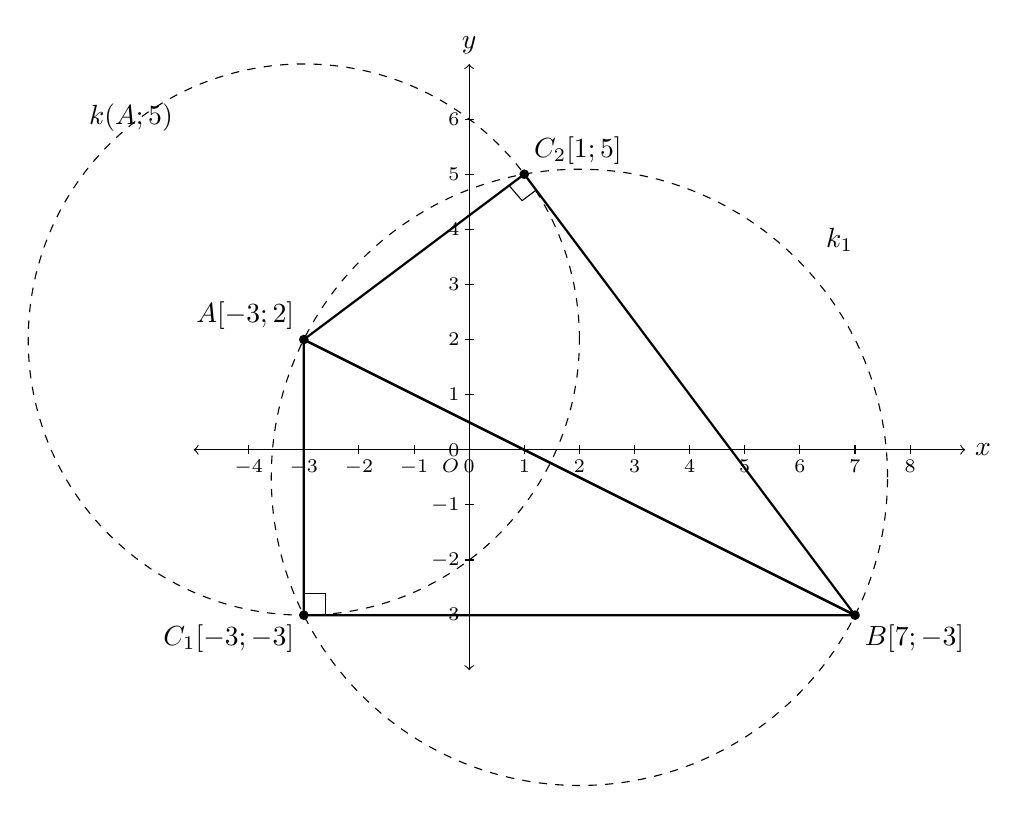
\begin{tikzpicture}[scale=0.7]

            % Osy
            \draw[<->, thin] (-5,0) -- (9,0) node[right] {$x$};
            \draw[<->, thin] (0,-4) -- (0,7) node[above] {$y$};
            \node[below left, font=\scriptsize] at (0,0) {$O$};

            % Značky na osách
            \foreach \x in {-4,-3,...,8}
            {
                \draw (\x,0.08) -- (\x,-0.08);
                \node[below, font=\scriptsize] at (\x,0) {$\x$};
            }

            \foreach \y in {-3,-2,...,6}
            {
                \draw (0.08,\y) -- (-0.08,\y);
                \node[left, font=\scriptsize] at (0,\y) {$\y$};
            }

            % Body
            \coordinate (A) at (-3,2);
            \coordinate (B) at (7,-3);
            \coordinate (C1) at (-3,-3);
            \coordinate (C2) at (1,5);
            \coordinate (M) at (2,-0.5);

            % Kružnice
            \draw[dashed] (A) circle (5);
            \draw[dashed] (M) circle ({sqrt(125)/2});

            % Trojúhelníky
            \draw[thick] (A) -- (B) -- (C1) -- cycle;
            \draw[thick] (A) -- (B) -- (C2) -- cycle;

            % Pravé úhly
            \draw (-3,-2.6) -- (-2.6,-2.6) -- (-2.6,-3);
            \draw (0.72,4.8) -- (0.96,4.52) -- (1.2,4.7);

            % Body
            \fill (A) circle (2.5pt) node[above left] {$A[-3;2]$};
            \fill (B) circle (2.5pt) node[below right] {$B[7;-3]$};
            \fill (C1) circle (2.5pt) node[below left] {$C_1[-3;-3]$};
            \fill (C2) circle (2.5pt) node[above right] {$C_2[1;5]$};

            % Popisky kružnic
            \node[above left] at (-5.2,5.6) {$k(A;5)$};
            \node[below right] at (6.3,4.2) {$k_1$};

        \end{tikzpicture}
        \caption{Body $C_1$ a $C_2$, pro které je trojúhelník $ABC$
        pravoúhlý s přeponou $AB$ a zároveň platí $|AC|=5$.}
        \label{fig:Right_triangle_given_hypotenuse_and_side}
    \end{figure}
\end{example}